\chapter{Codifica}
\label{cap:codifica}
\renewcommand{\lstlistingname}{Listato}

\intro{In questo capitolo viene descritto il processo di codifica del progetto di stage.}

\section{Codifica back-end}

Per approcciarmi alla codifica del progetto di stage, sono partito con la
definizione delle configurazioni: questo è stato il primo passo verso la
creazione del servizio.

\subsection{Config}

All'interno di questa cartella è presente il file di configurazione utilizzato
dal servizio. In questo file sono state inserite delle variabili d'ambiente, il
metodo più semplice all'interno di una funzione \emph{Lambda} per recuperare i nomi delle tabelle \emph{DynamoDB}
e i nomi dei \emph{bucket S3} dove verranno scaricate e infine salvate le immagini.

\subsection{Clients}
Successivamente ho avuto la necessità di comunicare con i \emph{bucket} e i
\emph{database}. Per fare ciò ho implementato due tipi di \emph{client}, quelli
\emph{remote} e quelli \emph{local}. È stato molto utile dividere le
funzionalità dei \emph{client}, perché mi ha permesso di avere più flessibilità durante
la codifica dei test. Di seguito spiego più in dettaglio le differenze:
\begin{itemize}
      \item \textbf{remote}: sono le funzioni che utilizzano i \emph{client} di
            \emph{DynamoDB} e \emph{S3} per recuperare e salvare i dati nell'ambiente
            \emph{sandbox}. Queste funzioni utilizzano la configurazione di
            \emph{default} per accedere ai servizi \emph{AWS};
      \item \textbf{local}: sono le funzioni che utilizzano i \emph{client} di
            \emph{DynamoDB} e \emph{S3} per recuperare e salvare i dati nell'ambiente di
            \emph{test} in locale. Queste funzioni utilizzano una configurazione vuota,
            senza credenziali, che punta ad un \emph{endpoint} locale.
\end{itemize}

\subsection{DAL}

Una volta definiti i metodi per stabilire la comunicazione con le risorse
\emph{AWS}, è stato necessario definire un metodo per recuperare i dati da
queste risorse. Una prima idea è stata quella di gestire lo scambio di dati
attraverso l'utilizzo diretto di un \emph{client}. Questo approccio, seppur
molto semplice e diretto, poteva portare ad un accoppiamento eccessivo tra le
parti del servizio, oltre che ad una vasta ripetizione di codice per ogni
operazione effettuata. Per questo motivo, dopo un confronto con il tutor
aziendale, è stato deciso di utilizzare il \emph{design pattern} \emph{DAO} per
gestire l'accesso ai dati. Questo metodo, nonostante preveda comunque della
ripetizione di codice, permette di aggiungere un livello di astrazione tra le
due parti che devono comunicare, rendendo più semplice la gestione di eventuali
cambiamenti: non sarà più necessario modificare il servizio, ma basterà
modificare solamente il \emph{DAO}.

\subsubsection{\emph{client configuration DAO}}

Questo file contiene la struttura che definisce un \emph{DAO} per il recupero di
una configurazione di un cliente. La definizione della struttura si trova nel listato \ref{client-conf}.
\begin{lstlisting}[label=client-conf, caption={Struttura di una configurazione di un cliente},captionpos=b, language=go]
type ClientConfiguration struct {
        ConfigurationName string `dynamodbav:"ConfigurationName"`
        Width   string `dynamodbav:"Width"`
        Height  string `dynamodbav:"Height"`
        Quality int    `dynamodbav:"Quality"`
    }
\end{lstlisting}
L'attributo \emph{dynamodbav} permette al \emph{client} di \emph{DynamoDB} di
mappare i campi della struttura con i campi della tabella. Inizalmente, durante
lo sviluppo in locale, ho utilizzato l'attributo \emph{json}: una volta testato
il codice nell'ambiente \emph{sandbox} il servizio non riusciva più ad
identificare i campi della struttura costruita. Ricontrollando la documentazione
ho individuato il problema ed è stato risolto velocemente.

\subsubsection{\emph{conversions bucket DAO}}

Questo file contiene la struttura che definisce un \emph{DAO} per effettuare il
\emph{download} e l'\emph{upload} di un file da un \emph{bucket S3}. È risultato
semplice creare queste due funzioni, in quanto la documentazione e gli esempi di
\emph{AWS} hanno mostrato in maniera chiara come gestire le due operazioni. La funzione
di \emph{download} prende in input tre parametri:
\begin{itemize}
      \item \textbf{clientID:} identificativo del cliente che ha richiesto la
            conversione;
      \item \textbf{jobID:} identificativo della conversione;
      \item \textbf{filename:} nome del file da scaricare.
\end{itemize}

Viene individuato il file all'interno del \emph{bucket S3} delle immagini da convertire, che si trova nella
cartella specificata dal \emph{clientID}. Una volta individuato il file viene effettuata una
copia del file in un percorso locale e viene restituito il percorso del file
appena salvato.\\

La funzione di \emph{upload} prende in input due parametri:
\begin{itemize}
      \item \textbf{clientID:} identificativo del cliente che ha richiesto la
            conversione;
      \item \textbf{filename:} nome del file da caricare.
\end{itemize}
Ogni file nei \emph{bucket} viene
identificato da una \emph{ObjectKey}: questa chiave è arbitraria e viene
definita nel momento in cui si effettua il caricamento di un file. Nel nostro
caso è risultato più comodo inserire anche il \emph{clientID} all'interno della chiave,
poiché è stato possibile creare automaticamente una cartella con l'ID del cliente desiderato
in cui inserire le immagini. \\

\subsubsection{\emph{image conversion jobs DAO}}

Questo file contiene la struttura che definisce un \emph{DAO} per inserire le
specifiche di una conversione oppure per aggiornarle. La struttura è quella
definita nel listato \ref{job-dao}.
\newpage
\begin{lstlisting}[label=job-dao,caption=Struttura di un \emph{job} di una conversione,captionpos=b, language=go]
    type ImageConversionJob struct {
        ClientID       string `dynamodbav:"ClientID"`
        CreationDate   int64  `dynamodbav:"CreationDate"`
        ContentType    string `dynamodbav:"ContentType"`
        JobID          string `dynamodbav:"JobID"`
        EndDate        int64  `dynamodbav:"EndDate"`
        Status         Status `dynamodbav:"Status"`
        SourcePath     string `dynamodbav:"SourcePath"`
        TotalTime      int64  `dynamodbav:"TotalTime"`
        ConversionTime int64  `dynamodbav:"ConversionTime"`
        ErrorCause     string `dynamodbav:"ErrorCause"`
    }
\end{lstlisting}

Vengono salvate tutte le informazioni riguardanti la conversione, nello
specifico vengono salvati:
\begin{itemize}
      \item \textbf{ClientID:} identificativo del cliente che ha richiesto la
            conversione;
      \item \textbf{CreationDate:} data di inizio della conversione;
      \item \textbf{ContentType:} formato del file da convertire;
      \item \textbf{JobID:} identificativo della conversione;
      \item \textbf{EndDate:} data di fine della conversione;
      \item \textbf{Status:} stato della conversione. Può assumere tre valori: \emph{RUNNING}, \emph{COMPLETE} e \emph{ERROR};
      \item \textbf{SourcePath:} percorso del file da convertire;
      \item \textbf{TotalTime:} tempo totale della conversione, compreso il tempo
            di \emph{download} e \emph{upload};
      \item \textbf{ConversionTime:} tempo di conversione;
      \item \textbf{ErrorCause:} causa dell'errore, se presente.
\end{itemize}

Un esempio di come viene visualizzato un \emph{job} all'interno del
\emph{database DynamoDB} è il seguente:
\begin{figure}[H]
      \centering
      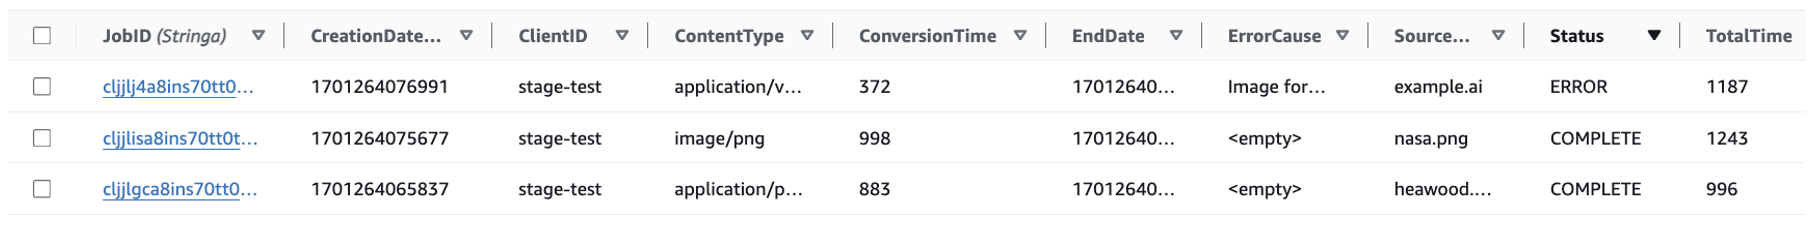
\includegraphics[width=1\textwidth]{images/esempio-job-dynamo.png}
      \caption{Esempio di un \emph{job} all'interno del \emph{database DynamoDB}}
\end{figure}


\subsection{Service}

Una volta preparate le risorse per gestire tutti gli aspetti della conversione,
si è reso necessario sviluppare il vero e proprio servizio di conversione.
Per gestire nella maniera più efficiente le conversioni, ho definito delle strutture che contengono tutti i formati gestiti dal
servizio, suddivisi per libreria che gestisce la conversione. Questi vengono
utilizzati per effettuare i controlli utilizzati come guardia per scegliere la
conversione adatta al formato richiesto. Questa scelta permette inoltre di
aggiungere con facilità nuovi formati di immagine, qualora il servizio che ha il
compito di convertirli sia stato aggiornato per supportarli. \\
Per accelerare il processo di
conversione, ho seguito il principio \emph{fail fast}: se il formato in ingresso
non è presente nelle strutture viene interrotto il flusso di conversione e viene restituito un
errore. Nella tabella contenente i \emph{job} di conversione, sarà presente
anche un campo dedicato a mostrare la causa dell'errore avvenuto.\\
Successivamente, se il formato è accettato, viene verificato se è in atto un tentativo di
\emph{upscaling} dell'immagine, confrontando le dimensioni dell'immagine con
quelle richieste dalla configurazione: se sta per essere effettuato, viene
saltata la conversione per quel formato e viene restituito un messaggio di
\emph{warning} per avvisare che quella conversione non verrà eseguita.\\
Viene effettuata la conversione utilizzando il metodo adatto al formato in
ingresso ed infine viene caricata l'immagine nel \emph{bucket} di output ed
aggiornata la tabella contenente i \emph{job} delle conversioni.\\
Questa è stata la parte principale del processo di codifica, che è stata molto
agevolata grazie allo sviluppo della \emph{PoC}: ho potuto riutilizzare le circa
cinquecento righe di codice scritte in precedenza per gestire tutte le
conversioni. Oltre alla parte delle conversioni ho dedicato del tempo a rendere
più pulito il codice, identificando le parti di codice ripetute e separandole
all'interno del file \emph{utils}, che definirò successivamente.

\subsection{Cmd}

Per eseguire il servizio appena descritto, è necessario un file che contiene la
vera e propria esecuzione della \emph{Lambda}. Nel file \emph{main.go} oltre
alle funzioni per gestire l'esecuzione del processo di conversione, è presente
la struttura che definisce un evento di conversione che viene definita nel
listato \ref{conversion-event}.
\begin{lstlisting}[label=conversion-event,caption={Struttura di un evento di conversione},captionpos=b, language=go]
    type ImageConversionEvent struct {
        Filename string `json:"filename"`
	ClientID string `json:"clientID"`
    }
\end{lstlisting}

Nello specifico vengono definiti:
\begin{itemize}
      \item \textbf{Filename}: nome del file da convertire;
      \item \textbf{ClientID}: identificativo del cliente che ha richiesto la
            conversione.
\end{itemize}
Entrambi vengono recuperati da un file \emph{JSON} che viene passato alla
funzione \emph{Lambda}: questo file nel progetto di stage viene inserito
manualmente, in un ambiente di produzione verrà fornito da un servizio
esterno.\\
Nella funzione \emph{main} viene scaricata dal \emph{database} la configurazione desiderata e
vengono istanziati i \glsfirstoccur\gls{DAO}, per poter
interagire con i servizi \emph{S3} e \emph{DynamoDB}. Infine viene
inizializzato il servizio che effettua la conversione delle immagini e viene
passato alla funzione \emph{Lambda}. \\
Tutte queste operazioni richiedono poche righe di codice grazie al pacchetto
\emph{SDK} fornito da \emph{AWS} per \emph{Go}: è stato molto semplice e diretto
scrivere il codice per questa parte del progetto.


\subsection{Utils}

Come accennato in precedenza, in questo file sono presenti le funzioni che devono svolgere compiti ripetitivi
oppure offrono metodi più semplici per interagire con programmi esterni alle
librerie di \emph{Go}. Ogni
funzione, se non specificato diversamente, ritorna sempre un errore nel caso in
cui le operazioni richieste non vadano a buon fine. Questo file è stato frutto
di una attività di \glsfirstoccur\gls{refactoring} del codice, che ha permesso
di
rendere più pulito il codice e di rendere più semplice la lettura dello stesso.
Le funzioni definite sono le seguenti:
\begin{itemize}
      \item \emph{ExecuteCommand:} questa funzione permette di eseguire un
            comando come se si fosse in un terminale, specificando il nome del
            programma da utilizzare e i parametri da passare. Viene utilizzata ogni
            volta che vengono invocati i programmi esterni alle librerie di \emph{Go};
      \item \emph{CheckUpscaling:} questa funzione permette di verificare se le
            immagini di input sono più piccole di quelle richieste in output. Se
            si sta per verificare un caso di \emph{upscaling}, viene
            \emph{loggato} un messaggio di \emph{warning} e viene ritornato un
            errore specifico;
      \item \emph{CheckFormat:} questa funzione ha lo scopo di verificare se il
            formato \glsfirstoccur\gls{mimetype}, che le viene passato come
            stringa, sia presente nella struttura contenente i formati accettati
            da una specifica conversione. Questa funzione viene riutilizzata per
            ogni formato e permette di identificare nella lista di stringhe,
            rappresentata come \emph{mappa}, se la chiave sia presente o meno.
            Ritorna un valore \emph{booleano} a seconda del risultato.
      \item \emph{GetImageSize:} questa funzione utilizza il percorso del file in
            esame per recuperare il peso in \emph{byte} dell'immagine e lo ritorna.
      \item \emph{RetrieveFormat:} questa funzione utilizza la funzione
            \emph{ExecuteCommand} per eseguire il programma \emph{Exiftool} con i
            parametri \emph{-s3}, \emph{-MIMEType}, \emph{filename}. Con questi
            parametri abbiamo indicato che vuole essere ritornato il \emph{mimetype} del
            file in esame nella forma abbreviata, grazie al parametro \emph{-s3}, che
            evita la stampa di descrizioni riguardanti il formato individuato.
      \item \emph{RetrieveResolution:} questa funzione, come la precedente,
            utilizza \emph{Exiftool} per recuperare la risoluzione dell'immagine in
            pixel. Viene utilizzata la forma abbreviata per la stampa delle informazioni
            e la stringa ritornata dal programma viene manipolata per ottenere le
            informazioni di larghezza e altezza come variabili separate.
      \item \emph{RetrieveResolutionEPS:} questa funzione, come la precedente,
            recupera la risoluzione dell'immagine in pixel, ma viene utilizzata per le
            conversioni di file di tipo \emph{EPS, PS} e \emph{AI}. Questi formati,
            essendo formati di tipo \emph{layered}, ossia caratterizzati da uno o più
            livelli, non sono facilmente interpretabili da \emph{Exiftool}. Per questo
            motivo viene utilizzato il comando \emph{identify} del programma
            \emph{ImageMagick}, che adempie al compito previsto.
      \item \emph{RetrieveColorSpace:} questa funzione utilizza \emph{Exiftool} e
            i parametri \emph{-s3}, \emph{-ColorSpace}, \emph{filename} per recuperare
            lo spazio colore utilizzato dall'immagine. Nel caso in cui questo comando
            ritorni il valore \emph{Uncalibrated}, viene rieseguito il \emph{Exiftool},
            questa volta con il comando \emph{-ColorSpaceData}, al fine di identificare
            lo spazio colore generale che è stato utilizzato.
      \item \emph{RescaleImage:} questa funzione utilizza la libreria \emph{vips}
            per eseguire la trasformazione dell'immagine, seguendo la larghezza e la
            altezza impostati come parametri. Viene restituito un tipo
            \emph{*vips.ImageRef}, ossia un puntatore ad un oggetto immagine gestito da
            \emph{vips}, su cui possono essere applicate altre trasformazioni prima di
            eseguire il salvataggio su file.
      \item \emph{TransformICCProfile:} questa funzione utilizza \emph{vips} per
            applicare il profilo colore desiderato all'immagine. Sono utilizzati due
            profili colore, uno di tipo \emph{sRGB} per tutti i profili colore
            individuati, mentre l'altro viene utilizzato per le immagini che utilizzano
            un profilo colore di tipo \emph{CMYK}: questo viene fatto per mantenere una
            rappresentazione uniforme dei colori a schermo.
      \item \emph{SaveImage:} questa funzione permette il salvataggio su file
            dell'immagine elaborata. Esistono due metodi per salvare l'immagine, a
            seconda del formato di output desiderato, quindi \emph{JPG} o \emph{PNG}.
            Ogni modalità di esportazione ha diversi parametri che possono essere
            impostati a piacimento, tuttavia nel progetto di stage l'unico parametro che viene
            utilizzato è quello relativo alla qualità dell'immagine, impostata in
            precedenza nella configurazione del cliente.
      \item \emph{CalculateNewResolution:} questa funzione viene utilizzata dalla
            conversione dei formati \emph{PSD}. Per questi file vi è la necessità di
            calcolare un fattore di \emph{scaling} per mantenere il rapporto prospettico
            dell'immagine, evitando eventuali deformazioni della stessa: questa operazione
            viene effettuata poiché la libreria utilizzata per gestire questi formati
            non effettua questo controllo.
            Il rapporto prospettico desiderato viene calcolato dividendo la larghezza desiderata per la larghezza originale
            dell'immagine e lo stesso viene fatto per l'altezza. Vengono poi confrontati
            i due fattori individuati e si utilizza quello più piccolo per effettuare la
            computazione della nuova risoluzione. Si effettua infine la moltiplicazione
            della larghezza e della altezza di input per il fattore di \emph{scaling}
\end{itemize}
